

\documentclass[journal,10pt,twocolumn]{article}
\usepackage{amsmath}
\usepackage{array}
\usepackage{booktabs}
\usepackage{amssymb}
\title{\textbf{Conics Assignment}}
\author{lakshmi kamakshi}
\date{September 2022}

\begin{document}

\maketitle
\paragraph{\textit{Problem Statement} -An arch is in the form of a parabola with its axis vertical.The arch is 10m high and 5m wide at the base.How wide is it 2m from the vertex of the parabola?} \vspace{5mm}

\section*{Solution}


Given, the axis of parabola is vertical,
\\ it's equation will be:
\begin{equation}
  x^2 = 4ay
  \end{equation}
\begin{figure}[h]
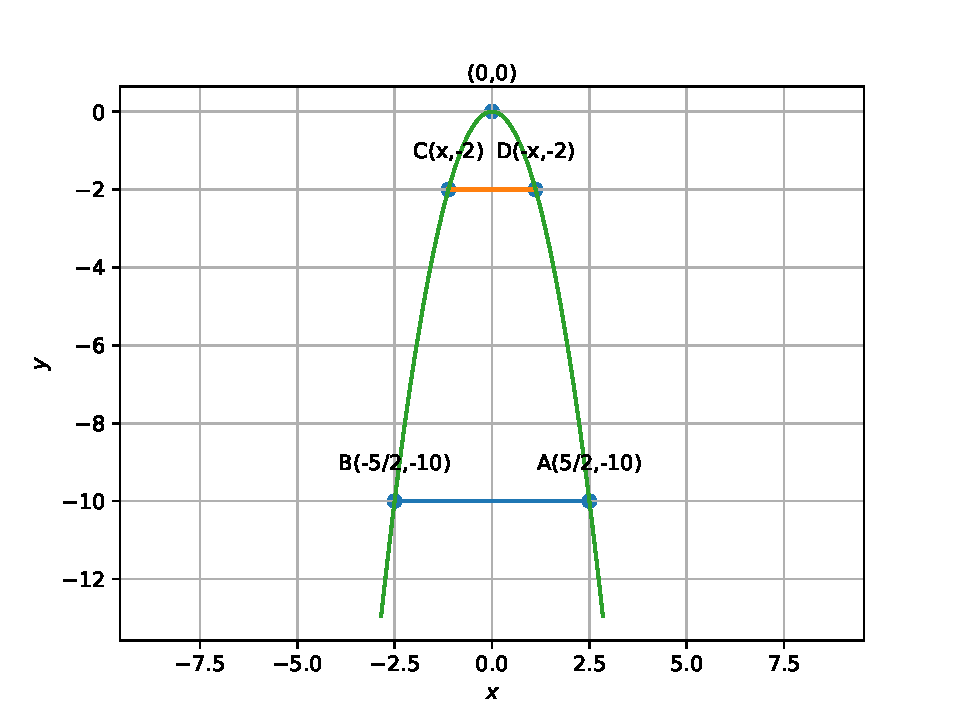
\includegraphics[width=1\columnwidth]{fig.pdf}
\end{figure}
\end{document}
